\chapter{Overview}
\label{cha:overview}

This chapter gives informal introduction to the RFSM language and of how to use it to describe 
FSM-based systems.

\medskip
Listing~\ref{lst:rfsm-gensig} is an example of a simple RFSM program\footnote{This program is
  provided in the distribution, under directory \texttt{examples/full/single/gensig}.}. This program is
used to describe and simulate the model of a calibrated pulse generator. Given an input clock
\verb|H|, with period $T_H$, it generates a pulse of duration $n \times T_H$ whenever input
\texttt{E} is set when event $H$ occurs.

\begin{lstlisting}[language=Rfsm,frame=single,numbers=left,caption=A simple RFSM
  program,label={lst:rfsm-gensig}]
@\label{gensig-1a}@fsm model gensig <n: int> (
  in h: event,
  in e: bool,
  out s: bool)
{
@\label{gensig-1}@  states: E0, E1;
@\label{gensig-3}@  vars: k: int<1:n>;
  trans:
  | E0 -> E1 on h when e=1 with k:=1, s:=1
@\label{gensig-4}@  | E1 -> E1 on h when k<n with k:=k+1
@\label{gensig-5}@  | E1 -> E0 on h when k=n with s:=0;
  itrans:
  | -> E0 with s:=0;
@\label{gensig-1b}@}

@\label{gensig-2a}@input H : event = periodic (10,0,80)
input E : bool = value_changes (0:0, 25:1, 35:0)
@\label{gensig-2b}@output S : bool 

@\label{gensig-6}@fsm g = gensig<3>(H,E,S)
\end{lstlisting}

\medskip
The program can be divided in four parts.

\medskip The first part (lines \ref{gensig-1a}--\ref{gensig-1b}) gives a \textbf{generic model} of
the generator behavior. The model, named \verb|gensig|, has one parameter, \verb|n|, two inputs,
\verb|h| and \verb|e|, of type \verb|event| and \verb|bool| respectively, and one output \verb|s| of
type \verb|bool|. Its behavior is specified as a reactive FSM with two states, \verb|E0| and
\verb|E1|, and one internal variable \verb|k|. The transitions of this FSM are given after the
\verb|trans:| keyword in the form :
\begin{center}
  \framebox{\lstinline[language=Rfsm]{| source_state -> destination_state on ev when guard with actions}}
\end{center}
where
\begin{itemize}
\item \emph{ev} is the event trigerring the transition,
\item \emph{guard} is a set of (boolean) conditions,
\item \emph{actions} is a set of actions performed when the transition is enabled.
\end{itemize}

The semantics is that the transition is enabled
whenever the FSM is in the source state, the event \emph{ev} occurs and all the conditions in the
guard are true. The associated actions
are then performed and the FSM moves to the destination state. For example, the first transition is
enabled whenever an event occurs on input \verb|h| and, at this instant, the value of input \verb|e|
is 1. The FSM then goes from state \verb|E0| to state \verb|E1|, sets its internal variable 
\verb|k| to 1 and its output \verb|s| to 1\footnote{Boolean values \texttt{true} and \texttt{false} can
  be denoted 1 and 0 respectively in programs.}.
   
\medskip
The \emph{initial transition} of the FSM is given 
after the \verb|itrans:| keyword in the form :
\begin{center}
  \framebox{\lstinline[language=Rfsm]{| -> initial_state with actions}}
\end{center}
Here the FSM is initially in state \verb|E0| and the output \verb|s| is set to 0.

\medskip
\textbf{Note}. In the transitions, the \lstinline[language=Rfsm]{when guard} and
\lstinline[language=Rfsm]{with actions} are optional and may be omitted.

\medskip
A graphical representation of the \verb|gensig| model is given in
Fig.~\ref{fig:rfsm-gensig-model} (this representation was automatically generated from the
program in Listing~\ref{lst:rfsm-gensig}, as explained in Chap.~\ref{cha:rfsmc}). 

\begin{figure}[!h]
   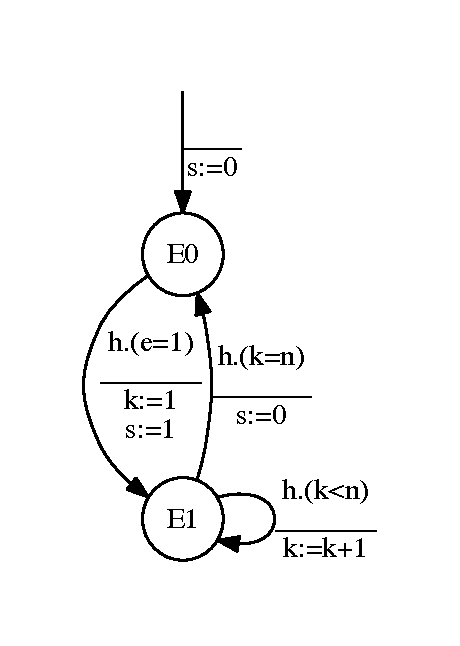
\includegraphics[height=9cm]{figs/gensig-model}
   \centering
  \caption{A graphical representation of FSM model defined in Listing~\ref{lst:rfsm-gensig}}
  \label{fig:rfsm-gensig-model}
\end{figure}

Note that, at this level, the value of the parameter \verb|n|, used in the type of the internal
variable \verb|k| (line~\ref{gensig-3}) and in the transition conditions (lines \ref{gensig-4} and
\ref{gensig-5}) is left unspecified, making the \verb|gensig| model a \emph{generic} one.

\medskip The second part of the program (lines \ref{gensig-2a}--\ref{gensig-2b}) lists \textbf{global inputs and
  outputs}.
% \footnote{In case of multi-FSM programs, this part will also contains the declaration of
%   \emph{shared} events and variables. See Sec.~\ref{sec:globals}.}.
For global outputs the
declaration simply gives a name and a type.  For global inputs, the declaration also specifies the
\textbf{stimuli} which are attached to the corresponding input for simulating the system. The
program of Listing~\ref{lst:rfsm-gensig} uses two kinds of stimuli\footnote{See
  Sec.~\ref{sec:inputs-outputs} for a complete description of stimuli.}. The stimuli attached to input
\verb|H| are declared as \emph{periodic}, with a period of 10 time units, a start time of 0 and a
end time of 80. This means than an event will be produced on this input at time 0, 10, 20, 30, 40,
50, 60, 70 and 80. The stimuli attached to input \verb|E| say that this input will respectively take
value 0, 1 and 0 at time 0, 25 and 35 (thus producing a ``pulse'' of duration 10 time units starting
at time 25).

\medskip
The third and last part of the program (line~\ref{gensig-6}) consists in building the global model of the system by
\emph{instanciating} the FSM model(s).
Instanciating a model creates a ``copy'' of this model for which
\begin{itemize}
\item the generic parameters (\verb|n| here) are now bound to actual values (3 here),
\item the inputs and outputs are connected to the global inputs or outputs. 
\end{itemize}

\medskip
A graphical representation of the system described in Listing~\ref{lst:rfsm-gensig} is given in
Fig.~\ref{fig:rfsm-gensig-top}\footnote{Again, this representation was actually automatically generated from the
program in Listing~\ref{lst:rfsm-gensig}, as explained in Chap.~\ref{cha:rfsmc}.}. 

\begin{figure}[!h]
   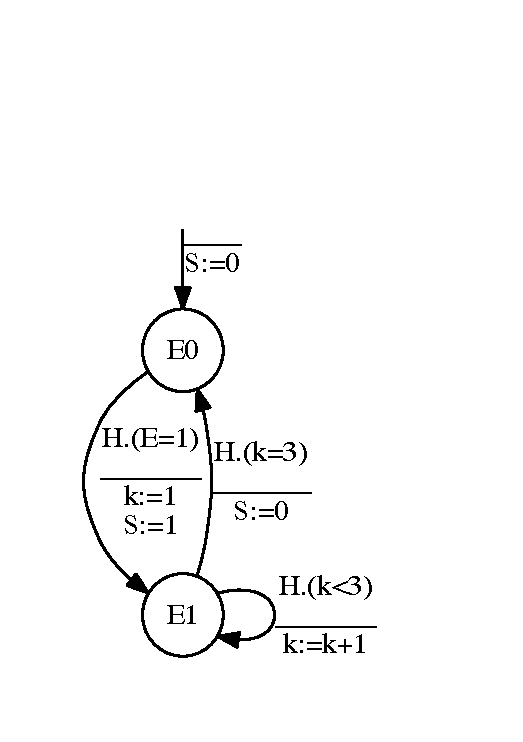
\includegraphics[height=7cm]{figs/gensig-top}
   \centering
  \caption{A graphical representation of system described in Listing~\ref{lst:rfsm-gensig}}
  \label{fig:rfsm-gensig-top}
\end{figure}

\section*{Simulating}
\label{sec:simulating-1}

Simulating the program means computing the reaction of the system to the input stimuli. Simulation
can be performed by the RFSM command-line compiler as described in chapter~\ref{cha:rfsmc}.
It produces a set of
\emph{traces} in VCD (Value Change Dump) format which can visualized using \emph{waveform viewers}
such as \texttt{gtkwave}. Some simulation results for the program in Listing~\ref{lst:rfsm-gensig}
are showed in Fig.~\ref{fig:rfsm-gensig-chrono}.

\begin{figure}[!h]
   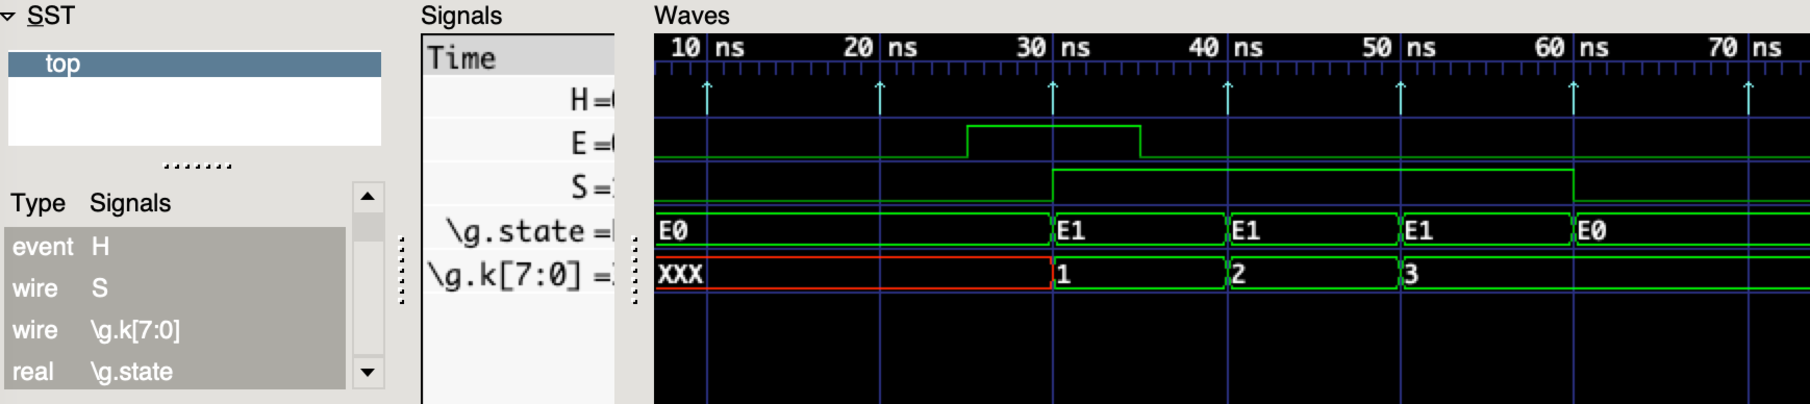
\includegraphics[width=\textwidth]{figs/gensig-chrono}
   \centering
  \caption{Simulation results for the program in Listing~\ref{lst:rfsm-gensig}, viewed using
    \texttt{gtkwave}}
  \label{fig:rfsm-gensig-chrono}
\end{figure}

\section*{Code generation}
\label{sec:code-generation-1}

RFSM can also generate code implementing the described systems simulation and/or
integration to existing applications.

\medskip
Currently, three backends are provided :
\begin{itemize}
\item a backend generating a C-based implementation of each FSM instance,
\item a backend generating a \emph{testbench} implementation in SystemC (FSM instances + stimuli
  generators),
\item a backend generating a \emph{testbench} implementation in VHDL (FSM instances + stimuli
  generators).
\end{itemize}

\medskip
The target language for the C backend is a C-like language augmented with
\begin{itemize}
\item a \verb|task| keyword for naming generated behaviors,
\item \verb|in|, \verb|out| and \verb|inout| keywords for identifying inputs and outputs,
\item a builtin \verb|event| type,
\item primitives for handling events : \verb|wait_ev()|, \verb|wait_evs()| and
  \verb|notify_ev()|. 
\end{itemize}
The idea is that the generated code can be turned into an application for a multi-tasking operating
system by providing actual implementations of the corresponding constructs and primitives.

\medskip
For the SystemC and VHDL backends, the generated code can actually be compiled and executed for
simulation purpose and. The FSM implementations generated by the VHDL backend can also be
synthetized to be implemented on hardware using hardware-specific tools\footnote{We use the
  \textsc{quartus} toolchain from Intel/Altera.}. 

\medskip
Appendices C1, C2 and C3 respectively give the C and SystemC code generated from the example in
Listing~\ref{lst:rfsm-gensig}. 

\section*{Variant formulation}
\label{sec:variant-formulation}

In the automata described in Fig.~\ref{fig:rfsm-gensig-model} and Listing~\ref{lst:rfsm-gensig}, the
value of the \texttt{s} output is specified by indicating how it changes when transitions are taken
(including its initialisation). This is typical of a so-called \emph{Mealy}-style description.  In
some cases, it is possible -- and maybe simpler -- to indicate which value this output takes for
each state. A equivalent description of that given
in Listing~\ref{lst:rfsm-gensig} is obtained, for example, by specifying that \texttt{s} is 0
whenever the FSM is in state \texttt{E0} and 1 whenever it is in state \texttt{E1}.
This style of description, often called
\emph{Moore}-style, is illustrated in Fig.~\ref{fig:rfsm-gensig-moore}. The value of the \texttt{s}
output is here attached to states using the \texttt{where} clause in the declarations of states.

\begin{figure}[htbp]
  \centering
  \begin{tabular}[c]{cc}
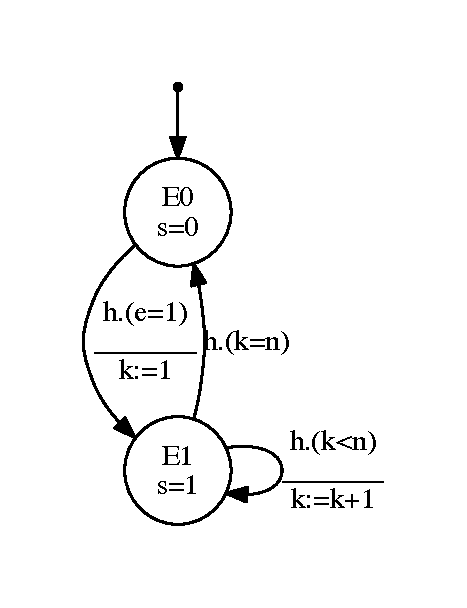
\includegraphics[width=0.4\textwidth]{figs/gensig-model-moore} &
\begin{minipage}[b]{0.6\textwidth}
\begin{lstlisting}[language=Rfsm]
fsm model gensig <n: int> (
  in h: event,
  in e: bool,
  out s: bool)
{
  states: E0 where s=0, E1 where s=1;
  vars: k: int<1:n>;
  trans:
  | E0 -> E1 on h when e=1 with k:=1
  | E1 -> E1 on h when k<n with k:=k+1
  | E1 -> E0 on h when k=n
  itrans:
 | -> E0 with s:=0
}
\end{lstlisting}
\end{minipage}
  \end{tabular}
  \caption{A reformulation of the model given in Listing~\ref{lst:rfsm-gensig} and
    Fig.~\ref{fig:rfsm-gensig-model} using Moore-style}
  \label{fig:rfsm-gensig-moore}
\end{figure}

\medskip \textbf{Note}. The \texttt{rfsmc} compiler automatically transforms models using
Moore-style descriptions models using only Mealy-style ones.

% This option is
% automatically inserted when simulating a system\footnote{\emph{I.e.} simulation is always performed
%   on Mealy-style FSMs.}. 

\section*{Multi-FSM models}
\label{sec:multi-fsm-models}

It is of course possible to describe systems composed of several FSM instances.

\medskip
A first example is given in Listing~\ref{lst:rfsm-cntmod8} and Fig.~\ref{fig:rfsm-cntmod8}. The system is a simple modulo 8 counter, here
described as a combination of three event-synchronized modulo 2 counters\footnote{This program is
  provided in the distribution, under directory \texttt{examples/full/multi/ctrmod8}.}.

Here a single FSM model (\texttt{cntmod2}) is instanciated thrice, as \texttt{C0}, \texttt{C1} and
\texttt{C2}. These instances are synchronized using two \textbf{shared events}, \texttt{R0} and \texttt{R1}. 
Shared events perform \emph{instantaneous synchronisation}. When a FSM \emph{emits} such an event, all transitions
triggered by this event are taken, simultaneously with the emitting transition. In the system
described in Fig.~\ref{fig:rfsm-cntmod8}, for example, the transition of \texttt{C0}
(resp. \texttt{C1}) from \texttt{E1} to \texttt{E0} occurs triggers the simultaneous transition of
\texttt{C1} (resp. \texttt{C2) }from \texttt{E0} to \texttt{E1} and, latter of \texttt{C1}
(resp. \texttt{C2}) from \texttt{E1} to \texttt{E0}.

\begin{figure}
  \centering
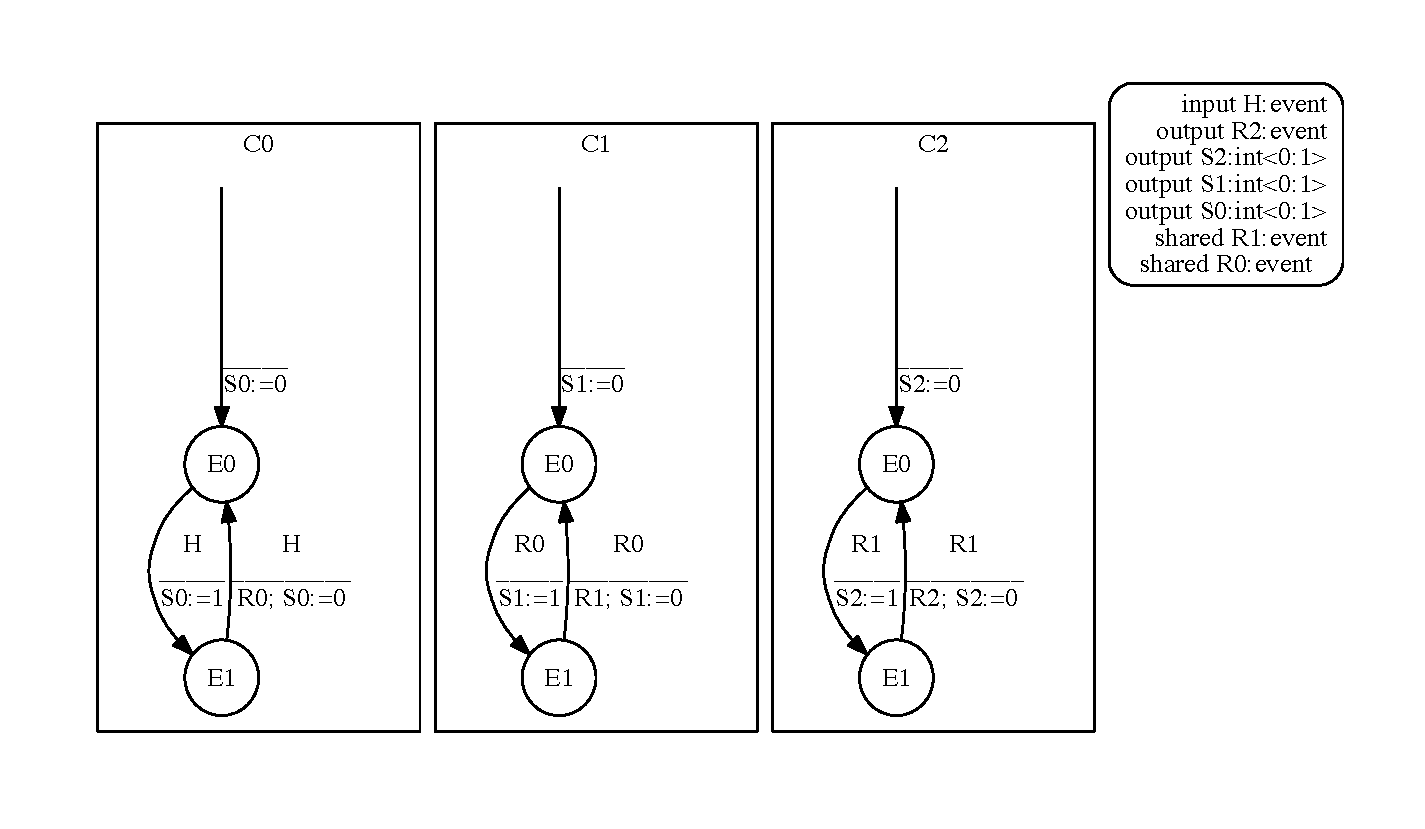
\includegraphics[width=\textwidth]{figs/ctrmod8-top}
  \caption{Graphical representation of the program of Listing~\ref{lst:rfsm-cntmod8}}
  \label{fig:rfsm-cntmod8}
\end{figure}

\begin{minipage}[c]{0.95\textwidth}
\begin{lstlisting}[frame=single,language=Rfsm,
  caption={A program involving three FSM instances synchronized by a shared event},
  label={lst:rfsm-cntmod8}]
fsm model cntmod2(
  in h: event,
  out s: bool,
  out r: event)
{
  states: E0 where s=0, E1 where s=1;
  trans:
  | E0 -> E1 on h
  | E1 -> E0 on h with r;
  itrans:
  | -> E0;
}

input H: event = periodic(10,10,100)
output S0, S1, S2: bool
output R2: event
shared R0, R1: event

fsm C0 = cntmod2(H,S0,R0) 
fsm C1 = cntmod2(R0,S1,R1) 
fsm C2 = cntmod2(R1,S2,R2) 
\end{lstlisting}
\end{minipage}

\pagebreak
Simulation results for this program are given in Fig.~\ref{fig:rfsm-cntmod8-vcd}.

\begin{figure}
   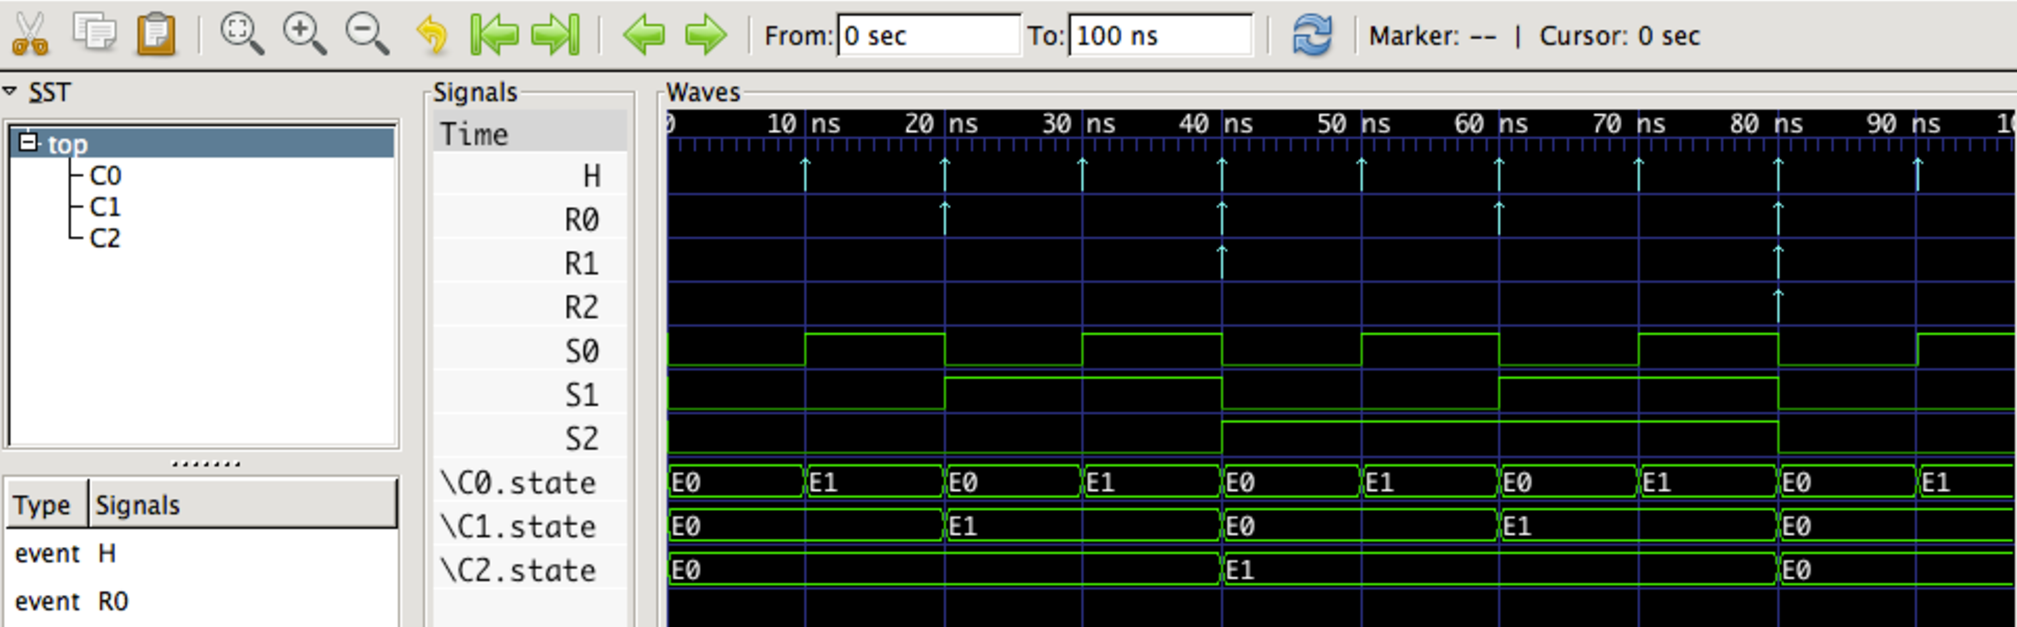
\includegraphics[width=0.9\textwidth]{figs/ctrmod8-chrono}
   \centering
  \caption{Simulation results for the program in Listing~\ref{fig:rfsm-cntmod8}}
  \label{fig:rfsm-cntmod8-vcd}
\end{figure}

\bigskip FSM instances can also interact by means of \textbf{shared variables}. This is illustrated
in Listing~\ref{lst:rfsm-shvar} and Fig.~\ref{fig:rfsm-shvar}\footnote{This program is provided in
  the distribution, under directory \texttt{examples/multi/synv_vp/ex5}.}. FSM \texttt{a1}
repeatedly writes the shared variable \texttt{c} at each event \texttt{h} so that it takes values 1,
2, 3, 4, 1, 2, \emph{etc}. FSM \texttt{a2} observes this variable also at each event \texttt{h} and
simply goes from state \texttt{S1} to state \texttt{S2} (resp. \texttt{S2} to \texttt{S1}) when the
observed value is 4 (resp. 1).

\begin{lstlisting}[frame=single,language=Rfsm,caption={A program involving two FSM instances and a
    shared variable},label={lst:rfsm-shvar}]
fsm model A1( in h: event, inout v: int)
{
  states: S1, S2;
  trans:
  | S1 -> S2 on h with v:=1
  | S2 -> S2 on h when v<4 with v:=v+1
  | S2 -> S1 on h when v=4;
  itrans:
  | -> S1 with v:=0;
}

fsm model A2( in h: event, in v: int)
{
  states: S1, S2;
  trans:
  | S1 -> S2 on h when v=4
  | S2 -> S1 on h when v=1;
  itrans:
  | -> S1 ;
}

input h : event = periodic(10,10,100)
shared c : int
fsm a1 = A1(h,c)
fsm a2 = A2(h,c)
\end{lstlisting}

\begin{figure}
  \centering
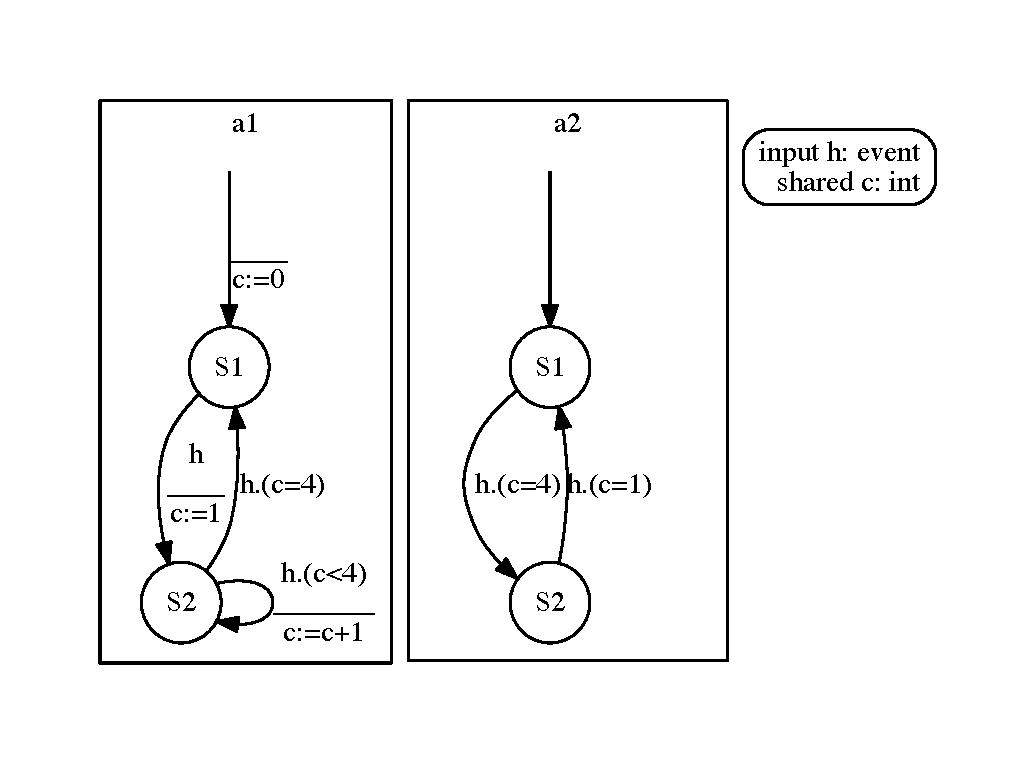
\includegraphics[width=0.8\textwidth]{figs/shvar-top} 
  \caption{Graphical representation of the program of Listing~\ref{lst:rfsm-shvar}}
  \label{fig:rfsm-shvar}
\end{figure}

Simulation results for this program are given in Fig.~\ref{fig:rfsm-shvar-vcd}.

\begin{figure}
   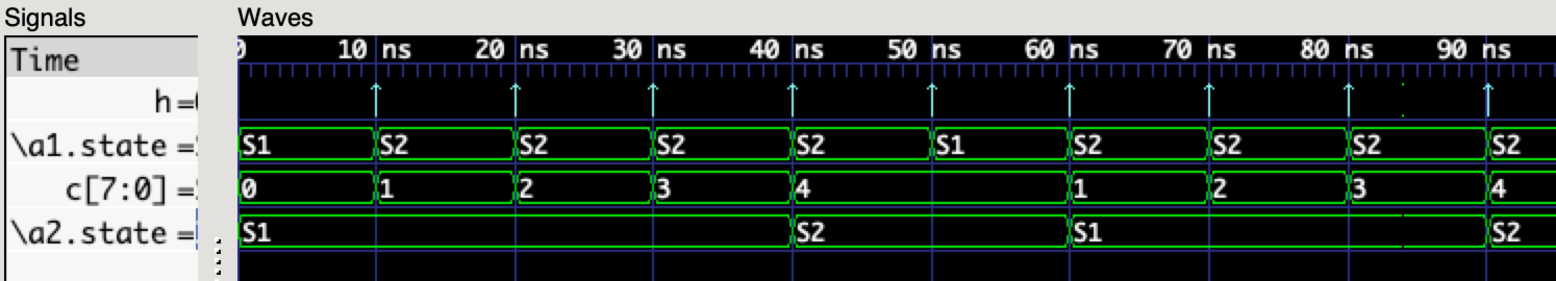
\includegraphics[width=0.95\textwidth]{figs/shvar-chrono}
   \centering
  \caption{Simulation results for the program in Listing~\ref{fig:rfsm-shvar}}
  \label{fig:rfsm-shvar-vcd}
\end{figure}


%%% Local Variables: 
%%% mode: latex
%%% TeX-master: "rfsm"
%%% End: 
